\documentclass[10pt,t]{beamer}
\usepackage[utf8]{inputenc}
\usepackage[T1]{fontenc}
\usepackage{graphicx}
\usepackage{grffile}
\usepackage{longtable}
\usepackage{wrapfig}
\usepackage{rotating}
\usepackage{amsmath}
\usepackage{textcomp}
\usepackage{amssymb}
\usepackage{capt-of}
\usepackage{hyperref}
\usetheme{default}

% ---------------------------------------------------------------------

\author{L. Larrabee Strow}
\date{\today}
\title{\large Radiometric Differences Between \newline
 AIRS, CrIS and IASI Derived for the  \newline
  CHIRP}
\subtitle{\footnotesize{AIRS Science Team Meeting}}
\date{\vspace{0.1in}\footnotesize{September 25, 2019 \vfill}}
\author{L. Larrabee Strow\inst{1,2}, C. L. Hepplewhite\inst{1,2}, H.M.Motteler\inst{1,2}, Sergio DeSouza--Machado\inst{1,2}, S. Buczkowski\inst{1,2}}
\institute[UMBC]{\inst{1} UMBC Physics Dept. \and \inst{2}UMBC JCET}
\input beamer_setup
\usetheme{metropolis}
\metroset{titleformat title=allcaps}
\renewcommand{\UrlFont}{\small\tt}
\renewcommand*{\UrlFont}{\footnotesize}
\tolerance=1000
\RequirePackage{fancyvrb}
\DefineVerbatimEnvironment{verbatim}{Verbatim}{fontsize=\footnotesize}
\begin{document}

\maketitle
\addtobeamertemplate{block begin}{
  \setlength{\parsep}{0pt}
  \setlength{\topsep}{3pt plus 2pt minus 2.5pt}
  \setlength{\itemsep}{0pt plus 0pt minus 2pt}
  \setlength{\partopsep}{2pt}
}

% --------------------------------------------------------------------
\section{Overview}
\begin{frame}
  \frametitle{Overview of talk}
  \begin{itemize}
  \item Definition of the CHIRP
  \item Establish the framework for determining climate quality radiometric records from the different sensors.
  \item Attribute quality and uncertainty for each channel.
  \item Utilization of large data sets of overlapping observations to quantify radiometric offsets between the sensors.
  \item Examples of results for single footprint observations.
  \item Spatial \& temporal sampling are not covered here.
    
  \end{itemize}
\end{frame}

% ---------------------------------------------------------------------
\section{CHIRP}
\begin{frame}
  \frametitle{The Climate Hyperspectral Infra-red Radiance Product}
  \begin{itemize}
  \item Spectrally equivalent to CrIS in medium resolution (MSR)
    \begin{itemize}
    \item MSR = 0.8/0.6/0.4 cm OPD (LW/MW/SW resp.)
    \item FSR = 0.8/0.8/0.8 cm OPD
    \item NSR = 0.8/0.4/0.2 cm OPD
    \end{itemize}
    
  \item The total number of channels available to use depends on the overlap of the parent sensor, for example AIRS L1C with 2645 channels to the CrIS MSR with 1683 with two guard channels per band edge.
  \item Covers the time period from AIRS L1C data availability (Sep 2002) to the present, with a transition from AIRS to CrIS proposed on Sep 2016.
      \item After the transition date (Sep 2016) CrIS-NPP L1C data have been available in FSR resolution and therefore the translation to the MSR grid is straightforward and carrying quality data to CHIRP simpler.

  \end{itemize}
\end{frame}

% ---------------------------------------------------------------------
\begin{frame}
  \frametitle{The CHIRP cont.}
  \begin{itemize}
   \item Operational overlap between sensors is now considerable: AIRS:CrIS Since 2012, AIRS:IASI from 2007 etc.
  \item The AIRS L1C currently includes cleaned and filled channels, the CHIRP will use drift corrected AIRS spectral radiance.
  \item CHIRP channels will carry the AIRS L1C noise, quality flag and L1C processing information (up to the transition date).
    \item CHIRP will have the same stability characteristics as the parent sensor (AIRS before and CrIS after the transition date).
  \item The AIRS fill channels are used and the corresponding CHIRP channels retained but will be flagged for the user. (Refer to accompanying talk).

  \end{itemize}
\end{frame}

% ---------------------------------------------------------------------
\section{Data Sets}
\begin{frame}
  \frametitle{SNO and Global Random Data Sets}
  \begin{itemize}
  \item Simultaneous nadir overpass (SNO) sets of observations have been accumulated for each pair of sensors: AIRS\&CrIS (NPP and N20),  AIRS\&IASI (MetOp-A and B), CrIS\&IASI (two sets).
  \item SNOs by definition are very closely paired observations but are weighted to high latitudes.
  \item Global random observations are available for several years, include all view angles, capture all scene types,  and must be corrected for mean view angle differences.
  \item Global random sets are sampled so that equal areas have equal numbers of observations (uniformly weighted with latitude).
    \item Best estimates of sensor offsets are derived from SNOs and global random sets.
  \end{itemize}
\end{frame}

% ---------------------------------------------------------------------
\begin{frame}
  \frametitle{Different Coverage}
  \begin{itemize}
  \item SNOs availability is dependent upon the relationship between the orbits of the two spacecraft. AIRS\&Cris SNOs IASI\&CrIS SNOs are distributed as shown here:
  \end{itemize}

  \begin{center}
  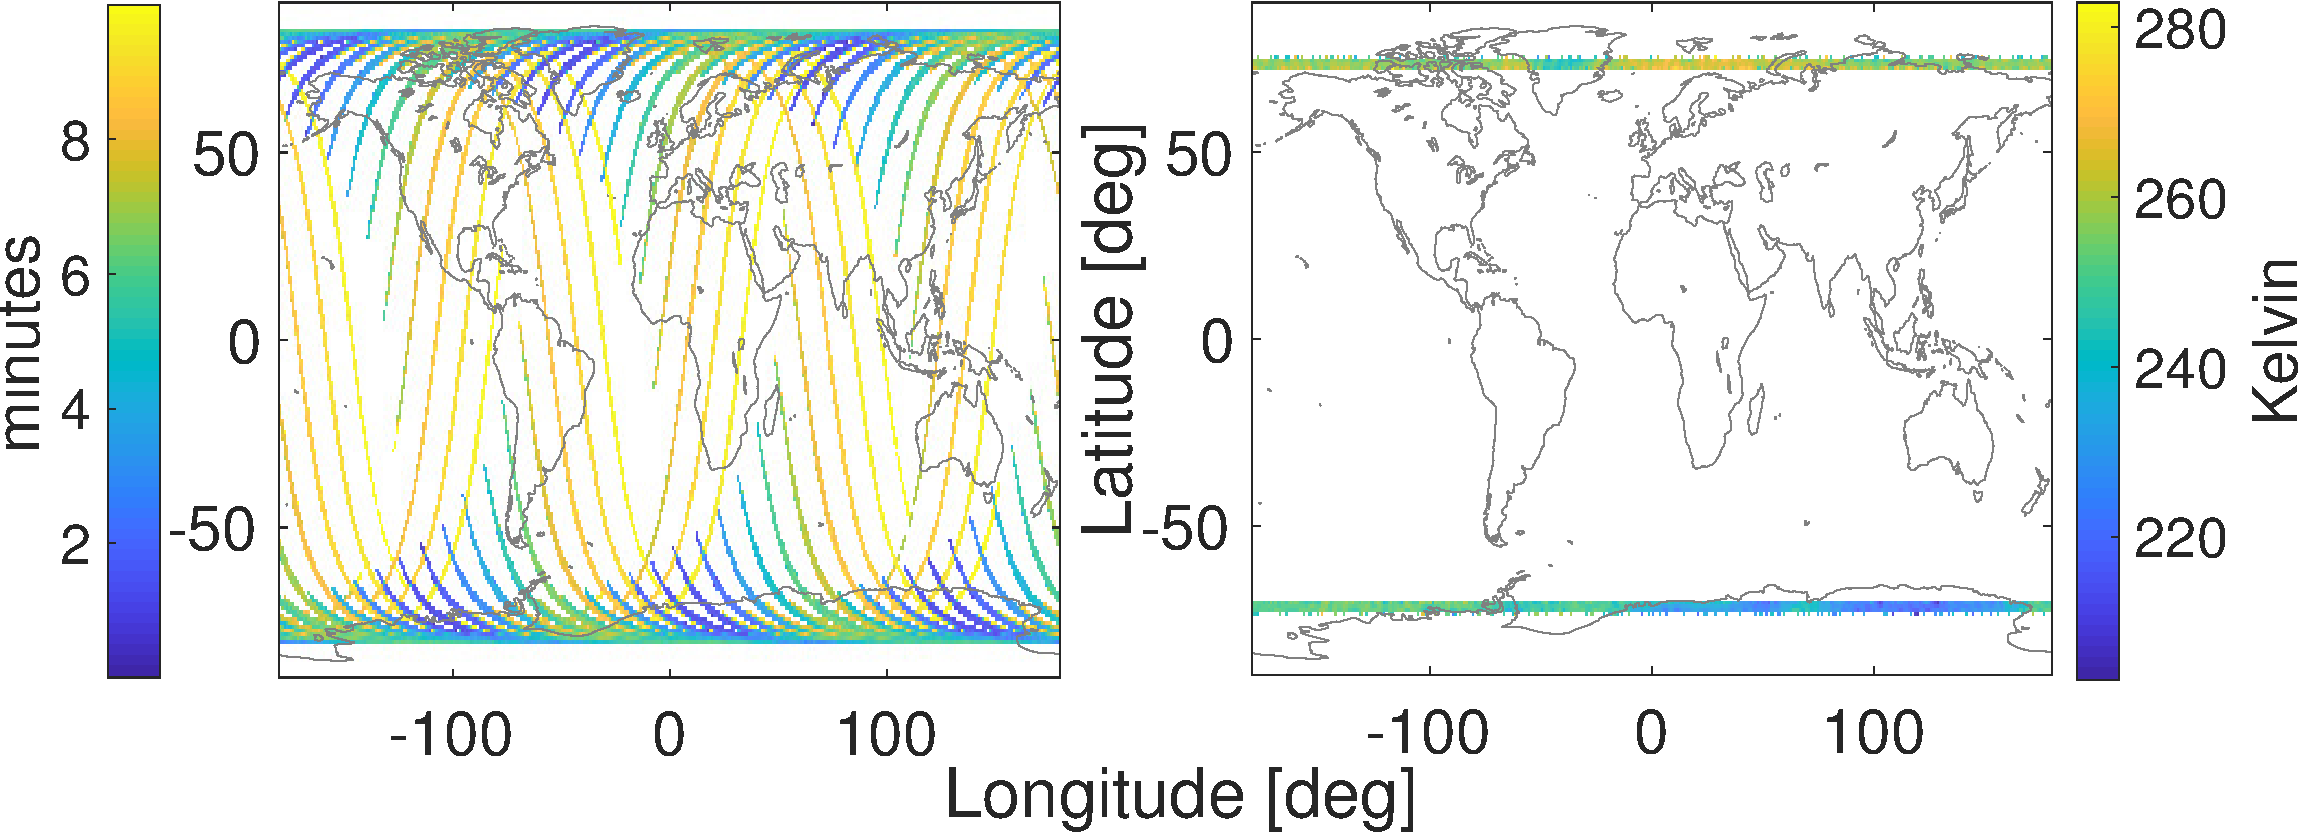
\includegraphics[width=\linewidth]{./Figs/Pdf/fig3_resize.pdf}
  \end{center}

\end{frame}

% ---------------------------------------------------------------------
\begin{frame}
  \frametitle{Different Samples}
  \begin{itemize}
  \item The different data sets cover slightly different ranges of scenes: more evident in the window channels than optically thick channels.
  \end{itemize}

  \begin{center}
    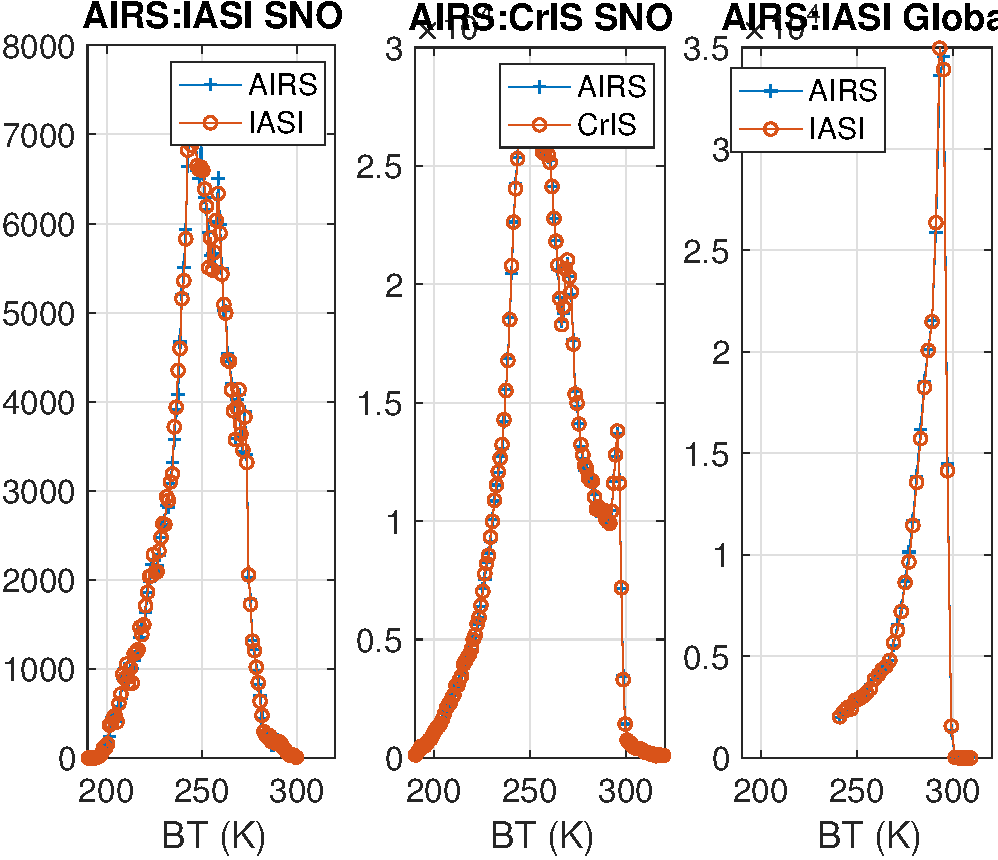
\includegraphics[width=0.66\linewidth]{./Figs/Pdf/Figsfig4_new.pdf}
  \end{center}

\end{frame}

% ---------------------------------------------------------------------
\section{Results}
\begin{frame}
  \frametitle{AIRS:CrIS SNOs}
  \begin{itemize}
  \item 2018 year of AIRS\&CrIS SNOs are compared on the CHIRP grid. About $1.5 x 10^6$ samples are acquired.
    \item AIRS L1C fill, dead and band edge channels are ommitted. The standard error of the mean is shown in the gray line.
  \end{itemize}

  \begin{center}
    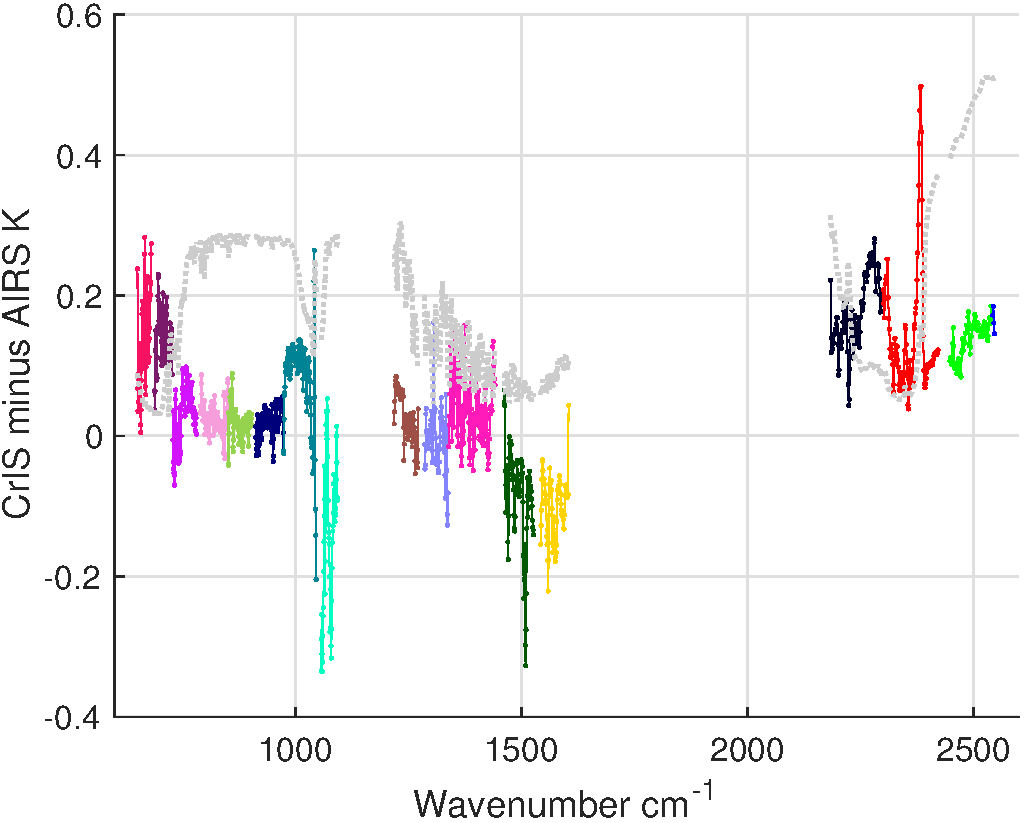
\includegraphics[width=0.66\linewidth]{./Figs/Pdf/ac_sno_2018_bias_stderr_coloraslp.pdf}
  \end{center}

\end{frame}

% ---------------------------------------------------------------------
\begin{frame}
  \frametitle{IASI:CrIS SNOs}
  \begin{itemize}
  \item 2017 year of IASI\&CrIS SNOs consists of about $7 x 10^4$ samples.
    \item Since IASI includes all CrIS bands, the resultant mean bias is computed for all CrIS channels. The standard error of the mean is shown in the gray line.
  \end{itemize}

  \begin{center}
    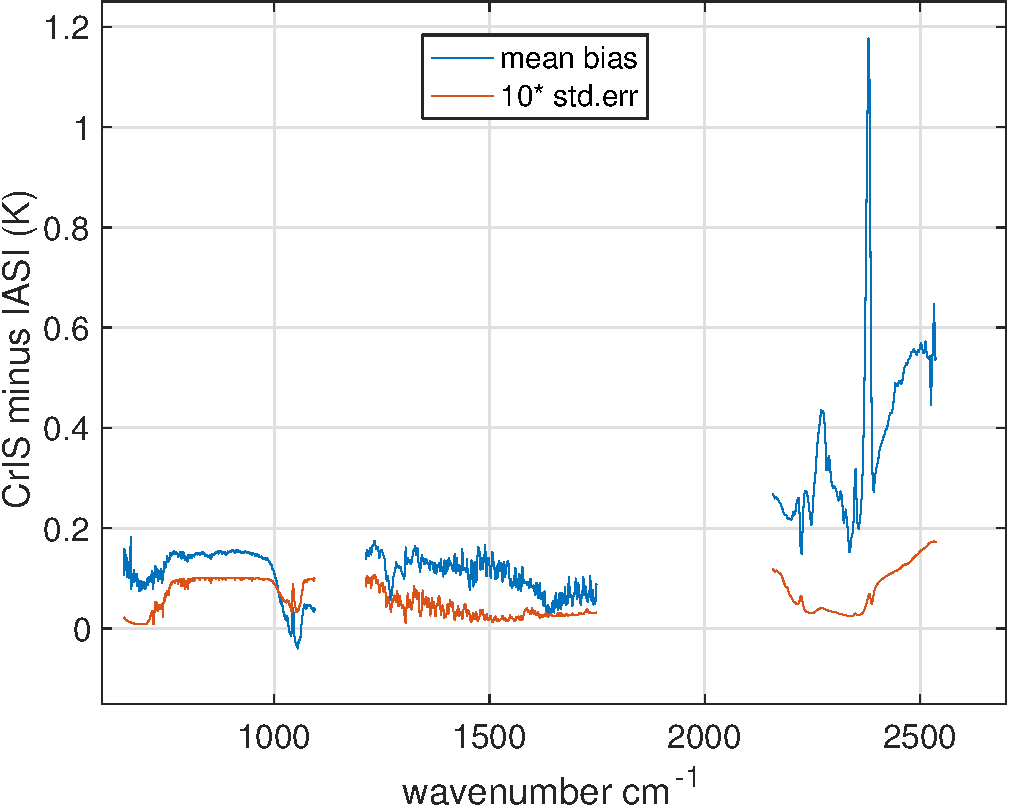
\includegraphics[width=0.66\linewidth]{./Figs/Pdf/ic_sno_nsr_2017_bias_stder_lw_mw_sw.pdf}
  \end{center}

\end{frame}

% ---------------------------------------------------------------------
\begin{frame}
  \frametitle{SNOs AIRS\&CrIS AIRS\&IASI on CHIRP}
  \begin{itemize}
  \item SNO pairs are collected for the complete period of operational overlap.
  \item Translation of AIRS L1C to CHIRP (CrIS MSR) and IASI to CHIRP permits both AIRS\&CrIS and AIRS\&IASI radiometric bias and then to use AIRS as the transfer when taking a double different to compute CrIS\&IASI bias.
  \item Every AIRS and IASI observation are first translated to CHIRP, then analysed.
  \item In the following figure the mean differences are computed for one year of data.
    \item The standard error of the mean is very similar to the individual SNO bias values shown previously.
  \end{itemize}
\end{frame}

% ---------------------------------------------------------------------
\begin{frame}
  \frametitle{SNOs AIRS\&CrIS AIRS\&IASI on CHIRP}
  
  \begin{center}
   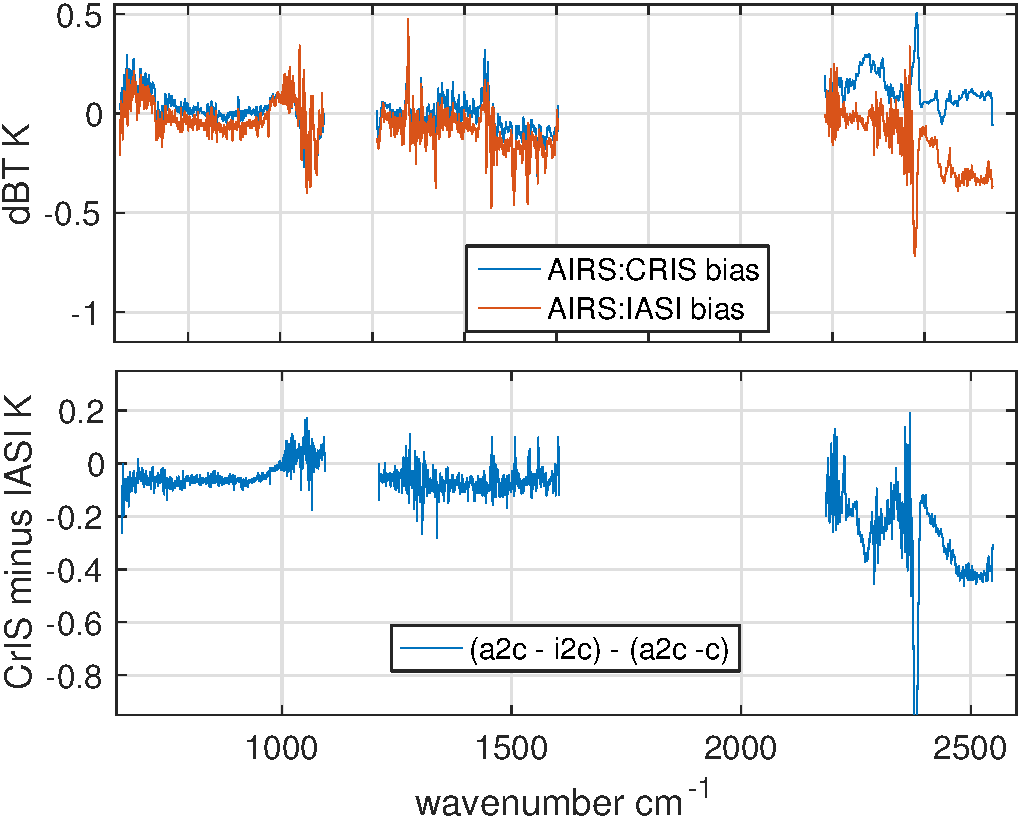
\includegraphics[width=0.8\linewidth]{./Figs/Pdf/ac_ai_2017_sno_msr_dble_diff_bias_aslp.pdf}
  \end{center}

\end{frame}

% ---------------------------------------------------------------------
\begin{frame}
  \frametitle{Global Random}
  \begin{itemize}
    \item 1\% of global random equal area samples returns about $1 x 10^7$ observations.
    \item Each AIRS observation is translated to the CHIRP (CrIS MSR) grid and compared to  CrIS on the same grid.
    \item The mean brightness temperature spectrum and mean difference is shown in the next figure. The standard error of the mean is negligible on this scale and is not shown.
      \item The small difference of the mean atmospheric view angle between the two sensors is corrected for each channel based on empirical correction derived from the data themselves.
    \item AIRS L1C fill channels, dead channels, and band-edge channels are not included.
      \item The different AIRS detector modules are distinguished by the different colors on the bias plot.
  \end{itemize}

\end{frame}
  
% ---------------------------------------------------------------------
\begin{frame}
  \frametitle{Gobal Random result}
  \begin{itemize}
    \item 2018 Global random on CHIRP
  \end{itemize}
  
  \begin{center}
    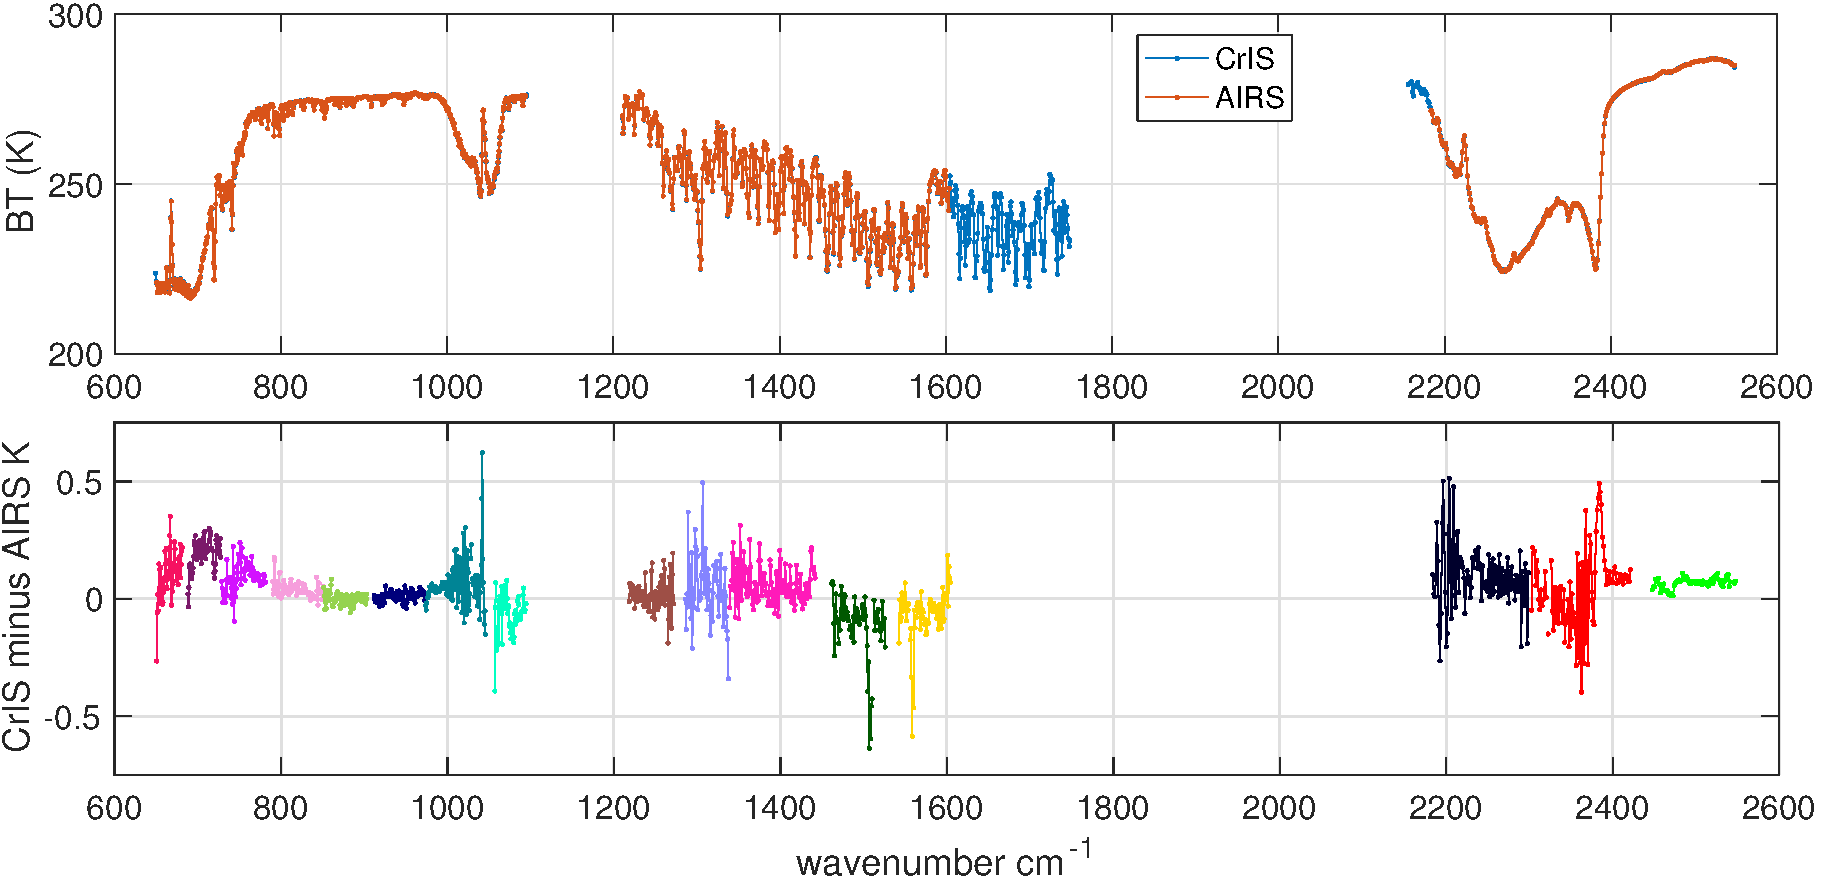
\includegraphics[width=\linewidth]{./Figs/Pdf/ac_global_random_fs_bias_mean.pdf}
  \end{center}

\end{frame}

% ---------------------------------------------------------------------
\section{Discussion \& Conclusions}
\begin{frame}
  \frametitle{}
  \begin{itemize}
  \item The translation algorithm of AIRS or IASI to the CHIRP (CrIS MSR) spectral grid has been demonstrated.
  \item Ref: H. E. Motteler and L. L. Strow, "AIRS Deconvolution and the Translation of AIRS-to-CrIS Radiances With Applications for the IR Climate Record," in IEEE Transactions on Geoscience and Remote Sensing, vol. 57, no. 3, pp. 1793-1803, March 2019.
  \item The SNO intercomparison provides a reliable means to quantify the bias as a function of wavelength.
    \item Using global random equal area samples over a full year gives consistent bias estimates as the SNO.
    \item The mean bias between the sensors is small, of order tenth Kelvin, and consistent across the band pass.
    \item The multi-year period of overlap of the missions has been used to determine the stability of the bias estimates with values close to the known AIRS drifts.
    
  \end{itemize}

\end{frame}

% ---------------------------------------------------------------------


\end{document}
